När Matlabb startas möts man av Matlabbs hjärta, Sök-vyn. Det är här
användaren söker efter och öppnar recept. Den enkla användaren behöver
bara trycka på \verb+sök+knappen och kan enkelt öppna det recept den är
intresserad av av recepten som dyker upp i listan. Mem det finns två
sätt att söka efter recept i matlabb, Titelsök och Filtersök.


\begin{figure}[h]
        \centering 
        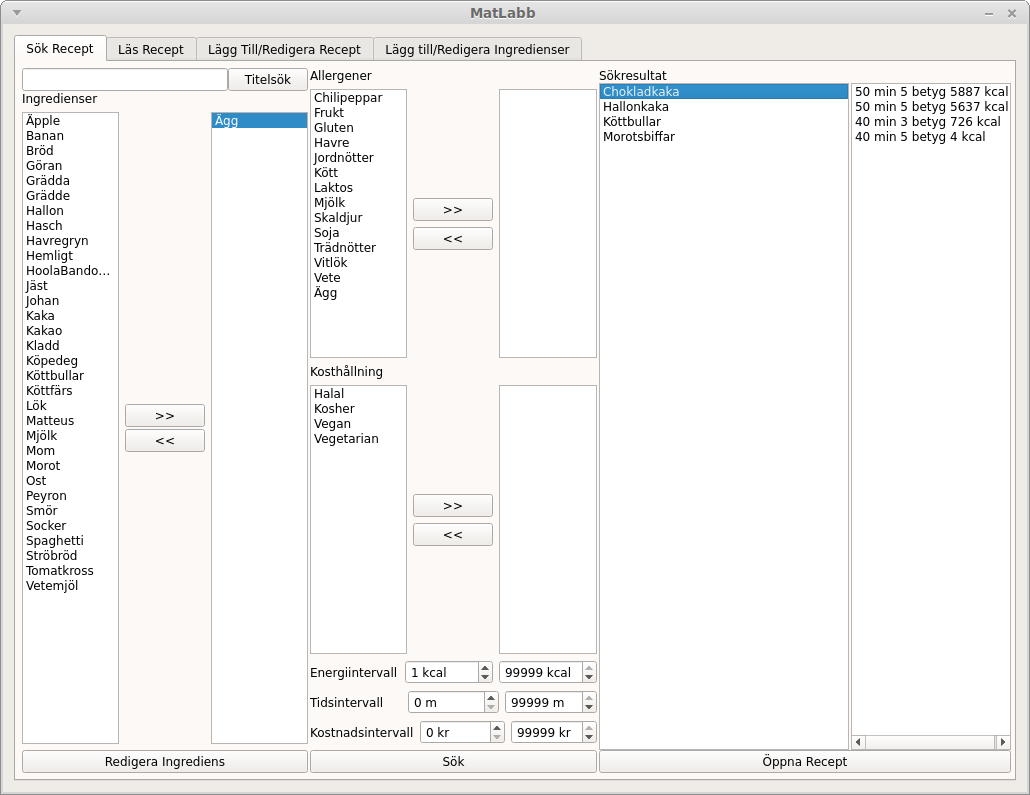
\includegraphics[scale=0.44]{sok_recept.png} 
        \caption{Sökvyn} 
        \label{fig:sokvyn}
\end{figure}


\subsection{Titelsökning}
Vet man redan vilket recept man är ute efter kan det enkelt och snabbt
hittas med hjälp av titelsökfunktionen. Receptets namn matas in i
titelsök rutan och hittas med \verb+titelsök+-knappen och kan sedan öppnas
med knappen \verb+Öppna+. Medans detta räcker för många kan även den
avancerade användaren istället filtrera sina sökningar.

\subsection{Filtersökning}

Matlabb har ett flertal avancerade filtreringsmekanismer, varav den
mest centrala är Ingrediensfiltrering. Ingrediensfiltret finns till
vänster i sök-vyn märkt Ingredienser. För att inkludera en ingrediens
i listan markeras den och flyttas till Sök-listan med hjälp av \verb+>>+
knappen. Vill man ta bort en ingrediens från sök-listan görs detta med
hjälp av \verb+<<+ knappen.

Till höger om Ingreienslistan ses två liknande listor. Genetiska
tillkortakommanden samt kosthållning som används för att filtrera bort
recept innehållande en viss allergen eller ifall man vill exkludera
recept av etiska eller religiösa skäl. Dessa fungerar på precis samma
sätt som för ingrediensfiltrering.

Under kosthållningslistan finns filtren för Energiinnehåll tidsåtgång
och portionskostnad. Filtreringen görs genom att med hjälp av pilarna
ange ett intervall om kommer begränsa sökningen till recept innom
intervallet.

När filtreringsinställningarna är färdiga slutförs sökningen genom att
knappen \verb+Sök+ trycks in och recepten dyker upp i listan till höger. För
att öppna ett recept markeras dess namn och när knappen \verb+öppna+ trycks
in skickas man vidare till recept-vyn.  

%section Receptvyn
I receptvyn möts man av en rad fält. I huvudfältet längst upp finner
man information om receptets namn antal kilokalorier per portion,
antal kronor per portion och hur lång tid receptet tar att laga.

Under huvudfönstret finns från vänster sett Ingrediensfältet,
instruktionsfältet samt kommentarsfältet. I ingrediensfältet finns de
ingredienser som krävs samt åtgångsmängd, i instruktionsfältet finns
instruktioner och i kommentarsfältet finns det möjlighet för korta
kommentarer ifall man inte önskar att ändra receptet.
